\section{Introduction}

Among all the tasks when designing a game, level design choices are some of the
most important \cite{blezinski2000, smith2008}. A well-designed level pushes a games' mechanics to its limits,
excites the player, and makes a good game great. A great example is the original
\emph{Super Mario Bros.} game. Only the first level sees the introduction of new
game mechanics, and afterwards new enemies are slowly introduced. However, the
number of units sold indicates that players found it to be a wortwhile and
rewarding game in sprite of the limited number of mechanics \cite{shaker2011}.

Level designers need to have knowledge across the spectrum of skills applicable
in game design \cite{blezinski2000}. They need an understanding of the game's mechanics, to know how
the artifical intelligence behaves, and to incorporate art assets into their 
levels in order to match the vision of the creative lead. Additionally, level
designers often have to switch between two considerations that constantly need
their attention: "Is this a good test of the skills that the player has
developed at this point in the game?" and "Does this obstacle fit with the
overall pacing and rhythm of the level?". Level designers frequentlly have to
use an iterative "modify and test" approach for certain game genres, as a small
change can sometimes have a large impact on the playability of a level \cite{smith2010}.

In spite of the importance of this task, the software for level designers has only
improved marginally over the years. In 2D games, the software is similar to many image
manipulation programs. For instance, in \emph{Super Mario Maker}'s level editor (which
can be seen in \autoref{fig:mm-editor}), the level designer drags terrain around with the resize and
translate handles, or uses drag and drop to place entities onto the map from a palette.
A similar comparison can be drawn for 3D level editors such as \emph{Trenchbroom}. In
Trenchbrrom, the level designer builds geometry as if they were creating a 3D model, then
moves around entities as they please. Level editing in both cases is a direct manipulation
task, but far too often level editors lack feedback that could help the designers more
quickly identify and correct mistakes, to the detriment of the efficiency and pleasure of
associated with level editing as a direct manipulation task \cite{schneiderman1983}. It is my
opinion that it would be more beneficial to the level designer if immediate feedback was 
provided on the level before playtesting begins, so problems could be eliminated as they
appear. One example would be to inform the level designer of levels that are not playable
before the designer runs playtesting. The need for better level editing tools is made
apparent by other software that has lowered the barrier for entry in the game development
industry such as the wide variety of open source game engines, intelligent development
environments, visual programming interfaces, and frameworks available to developers.

\begin{figure}[h]
    \centering
    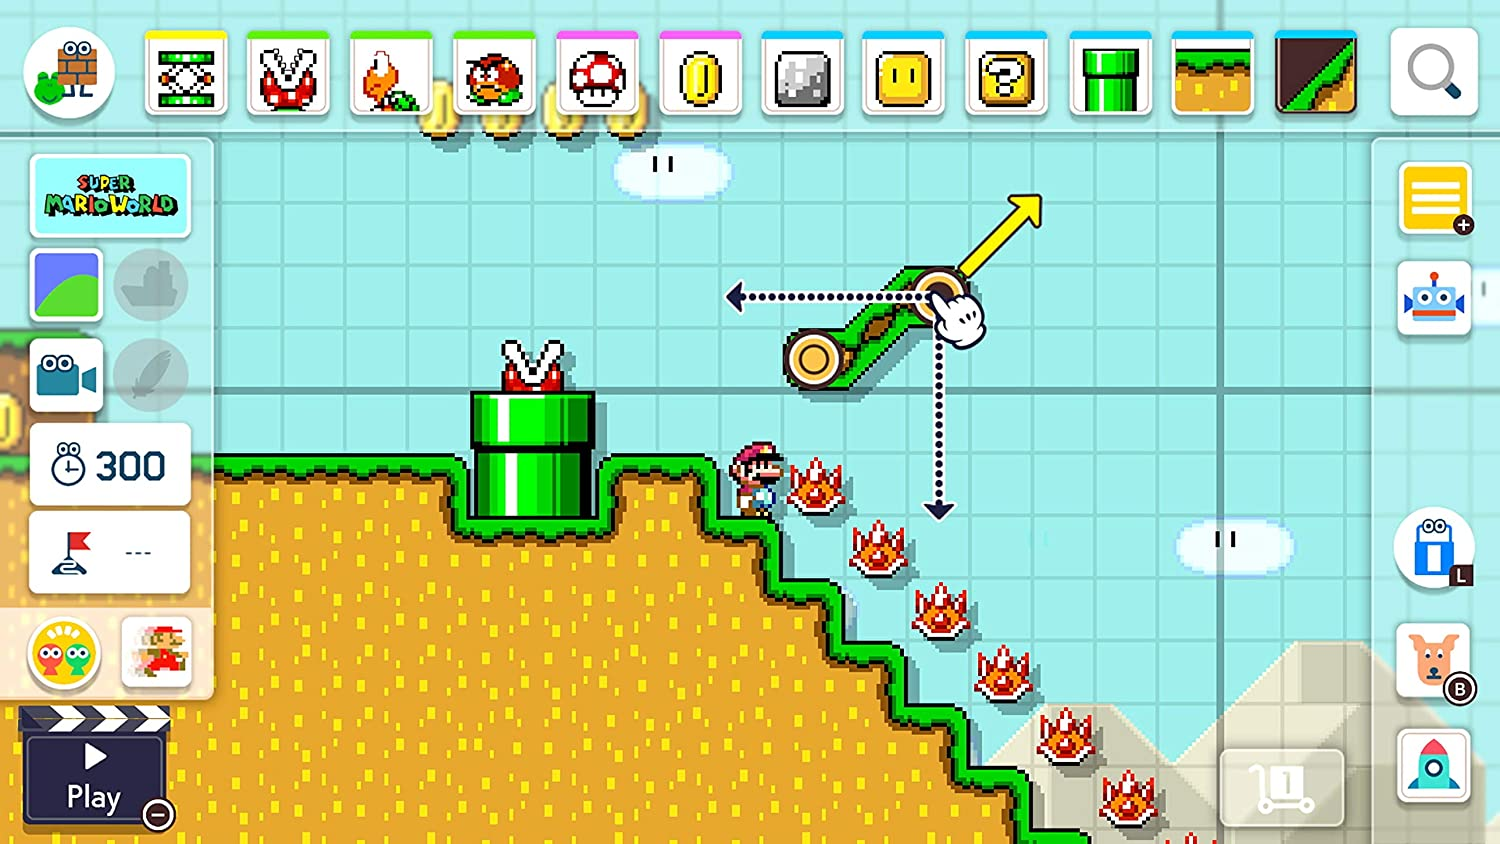
\includegraphics[width=0.8\textwidth]{img/fig1-mm-editor.jpg}
    \caption Interface of \emph{Super Mario Maker}'s level editor.
    \label{fig:mm-editor}
\end{figure}

One approach that is often implemented for level creation is procedural content generation.
Procedural content generation refers to the use of an algorithm to generate many kinds of
content \cite{shaker2016}. It has been used for terrain in 3D games like 
\emph{No Man's Sky}, dungeons in \emph{The Binding of Isaac}, complete worlds such as in
\emph{Endless Web} \cite{smith2013}, and even entire games like \emph{Yavalath}
\cite{browne2011}. Procedural content generaTion is a very versatile tool. One of the
motivations of the field is to create content much more quickly than ahuman can, and to
generate ideas that a human game designer may not have been able to come up with by
themselves. Procedural generation has been used in the past due to memory constraints - it
is more space efficient to store a single integer as a seed, and to generate a world at
runtime using it \cite{shaker2012}. \emph{Elite} used procedurally generated worlds to deal
with memory limitations. Roguelike games such as \emph{Hades}, and \emph{Risk of Rain 2}
commonly use procedural generation. The wide variety of encounters to explore due to the
stochastic nature of procedural content generation can be very engaging, and in the case of
games like \emph{Spelunky}, it can take hundreds of games to explore the entire procedural
space \cite{kazemi2011b}. In commercial platforming games, it is not very common to see
procedural generation used \cite{compton2006}, in spite of the increase in the amount of
content, replayability value, and development time saved by its use.

Shaker et al. describe a number of desirable properties of content generators \cite[6-7]{shaker2016}.
These properties include speed, controllability, reliability, expressivity and diversity,
and creativity. The importance of each property depends on the application. As an example,
a level generator that creates platform games at runtime needs to be fast. It needs to be
reliable so that there is a guaranteed route through a level. Additionally, it should be
creative, so that the levels it generates remain interesting over time.

Procedural content generation has been previously split into a taxonomy by Togelius et al.
\cite{togelius2011}, and this taxonomy is useful for describing content generators. The 
taxonomy is summarised in \autoref{table:pcg-taxonomy}. Level editing tools are one example
of offline content, and this category also includes games that ship with level editors.
Adapative content generation is present in \emph{Left 4 Dead}. The number and difficulty
of enemy encounters scale according to how well the players perform, so the content
generator adapts to different groups of players. Content generators that use evolutionary
algorithms or gramars make use of a generate and test approach, while chunk-based generation
approaches are normally constructive.

\begin{longtable}[c]{| c | c | c |}
\caption{Taxonomy of procedural content generation\label{long}}\\
\label{table:pcg-taxonomy}
\hline
Property of generator & \multicolumn{2}{| c |}{Possible values of property}\\
\hline
\endhead
Moment of content creation & Online - Content created during playtime & Offline - Content is either created separately, or during development.\\
\hline
Type of content & Necessary - The produced content is required to play the game. & Optional - The game is playable without the generated content.\\
\hline
Dimension of control & Random - The generator is not controllable by a user to any exten. & Parameterized - The user may set parameters which affect the generator's output.\\
\hline
Applicability & Generic - The generator's output can be used in many contexts, or is applied to many different conditions. & Adapative - The content of the genetor adapts to different conditions.\\
\hline
Reproducibility & Stochastic - Knowing the input conditions of the generator is not sufficient for prediciting the output. & Deterministic - KNowing the input conditions of the generator is sufficient to predict its output.\\
\hline
Level of authorship & Mixed - The generator may require or optionally use input from a user. & Automatic - The generator is capable of producing content autonomously.\\
\hline
Production approach & Generate and test - The generator constructs a large number of potential solutions and searches for an optimal selection. & Constructive - The generator sequentially constructs an acceptable solution.\\
\hline
\end{longtable}

Platformer games are often the subject of papers on level generation for video games. A
platformer is a set of physics-based dexterity challenges that are viewed from the side
\cite{shaker2011}. The player navigates their avatar past obstacles, collects currency,
defeats enemies, and proceeds to the end of the level. Platformer games often have many 
short levels that the player must complete before finishing the game. These levels are
often time restricted, may or may not have checkpoints, and often implement a system where
the player can make a finite number of mistakes before having to restart from the beginning,
as is the case for both Super Mario Bros. and \emph{Crash Bandicoot}. In some game genres,
it is a challenge to evaluate the difficulty of a task at a glance, but a player familiar
with a platformer game can quickly gauge the challenge presented by a task, as the hazards
need to be visible in order for the player to react to them adequately \cite{sorenson2010}.
As an example, given a level in Super Mario Bros., a player knows that falling down a pit 
will instantly kill them, and can reason that larger pits make for a greater challenge.
Computers do not have the same level of intuition that experienced human players have about
the task, and it can be difficult to model a player's behaviour to generate appropriate
levels for them \cite{shaker2011}, which makes procedural content generation for platformers
such an interesting undertaking. Furthermore, the rules and actions present in platformers
are often simple (for instance, the primary actions in Super Mario Bros. are running and
jumping), but creative level geometry and enemy placement can lead to a large variety of
enjoyable content, despite the limited actions \cite{dahlskog2012}.